
Los valores entregados son el promedio de las 3 muestras de cada configuración. Como cada variación entre las muestras fue baja (inferior al $4\%$ en todos los casos), no se incluyen barras de error. Cada figura se genera automáticamente con el script \texttt{plot\_generator.py} correspondiente; una copia queda en \path{code/sorting/data/plots/} y \path{code/matrix_multiplication/data/plots/}.

\subsection{Ordenamiento de arreglos}

Las implementaciones de Merge Sort y QuickSort se tomaron de GeeksforGeeks \cite{gfg_mergesort,gfg_quicksort}, la de Patience Sort de Rosetta Code \cite{rosetta_patience} y \texttt{std::sort} es la de la biblioteca estándar \cite{cppref_sort}. QuickSort se modificó para usar pivote aleatorio \cite[cap.~7]{clrs}.

\subsubsection{Tiempo de ejecución}

\begin{figure}[H]
    \centering
    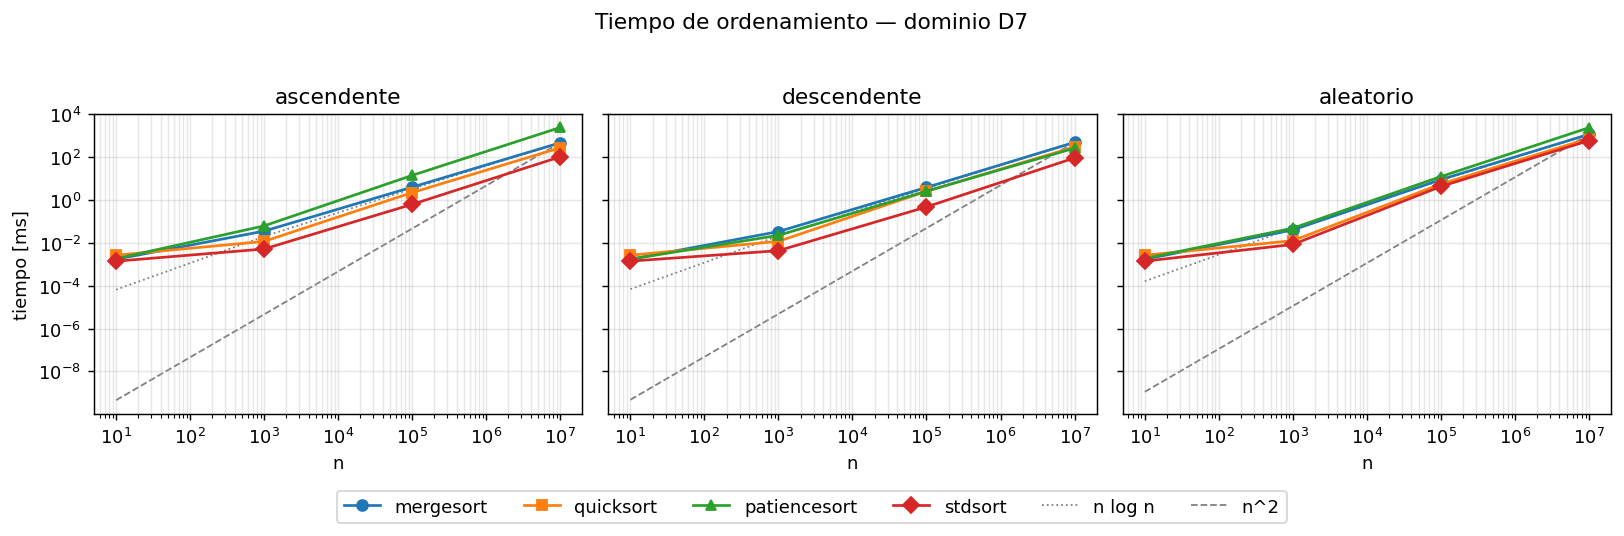
\includegraphics[width=0.95\textwidth]{sections/plots/sorting_tiempo_D7.png}
    \caption{Tiempo de ejecución promedio de los cuatro algoritmos de
    ordenamiento en el dominio $D_7 = \{0,\dots,10^7\}$, por tipo de entrada.
    Escala log--log; las líneas grises son las referencias $n\log n$ y $n^2$.}
    \label{fig:sort_time_d7}
\end{figure}

\begin{table}[H]
    \centering
    \begin{tabular}{r|rrrr|rrrr}
         & \multicolumn{4}{c|}{$D_1 = \{0,\dots,9\}$} & \multicolumn{4}{c}{$D_7 = \{0,\dots,10^7\}$} \\
        $n$ & Merge & Quick & Patience & \texttt{std} & Merge & Quick & Patience & \texttt{std} \\ \hline
        $10^3$ & 0.039 & 0.041 & 0.037 & 0.006 & 0.039 & 0.012 & 0.047 & 0.008 \\
        $10^5$ & 5.81 & \textbf{235.2} & 4.97 & 1.52 & 8.75 & 5.44 & 12.09 & 4.18 \\
        $10^7$ & 636 & \textbf{---} & 487 & 172 & 1125 & 722 & 2304 & 576 \\
    \end{tabular}
    \caption{Tiempo de ordenamiento [ms], entrada aleatoria. \textbf{---}: la
    corrida superó el límite de tiempo de 300 s.}
    \label{tab:sort_time}
\end{table}

Con respecto a $D_7$ (\cref{fig:sort_time_d7}, \cref{tab:sort_time}), todos siguen la pendiente de $n\log n$. Sin embargo, podemos ver que \texttt{std::sort} es el más rápido y el Patience Sort es el más lento para $n$ grande (2304 ms vs 576 ms de \texttt{std::sort} a $n=10^7$).
Podemos ver también que los factores de crecimiento medidos de $10^5$ a $10^7$ son $\times 129$ (Merge), $\times 133$ (Quick), $\times 138$ (\texttt{std}) y $\times 191$ (Patience), cercanos al $\times 140$ que predice $n\log n$. La desviación de Patience Sort se explica por su mayor constante y su peor localidad de memoria (reparto en pilas y mezcla con un heap).

\begin{figure}[H]
    \centering
    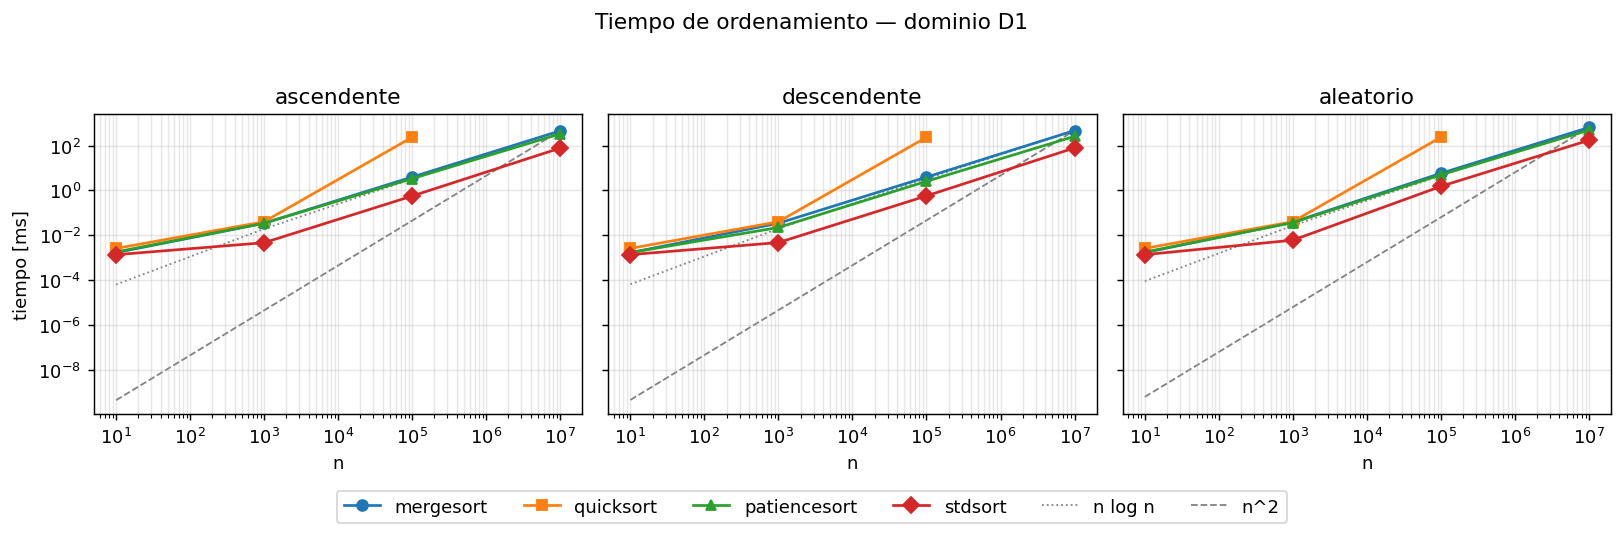
\includegraphics[width=0.95\textwidth]{sections/plots/sorting_tiempo_D1.png}
    \caption{Tiempo de ejecución promedio en el dominio $D_1 = \{0,\dots,9\}$.
    QuickSort se separa del resto y a $n=10^7$ no completa dentro del límite de
    tiempo (su curva termina en $n=10^5$).}
    \label{fig:sort_time_d1}
\end{figure}

El comportamiento cambia por completo en $D_1$ (\cref{fig:sort_time_d1}): QuickSort se curva hacia $n^2$ y a $n=10^7$ no termina. Ya a $n=10^5$ tarda 235 ms, unas $40$ veces más que Merge Sort.
La causa es la enorme repetición de valores: con solo $10$ valores distintos, tras unos pocos niveles de recursión un subarreglo queda formado por un único valor repetido, y la partición de Lomuto, con su comparación estricta ($<$), extrae un solo elemento por llamada, degradándose a $O(m^2)$. Como el pivote es aleatorio, esto no es el peor caso clásico de entrada ordenada (de hecho las entradas ascendente y descendente en $D_7$ terminaron sin problema), sino un efecto propio de los datos con muchos duplicados que ningún pivote corrige.


\subsubsection{Uso de memoria}

\begin{figure}[H]
    \centering
    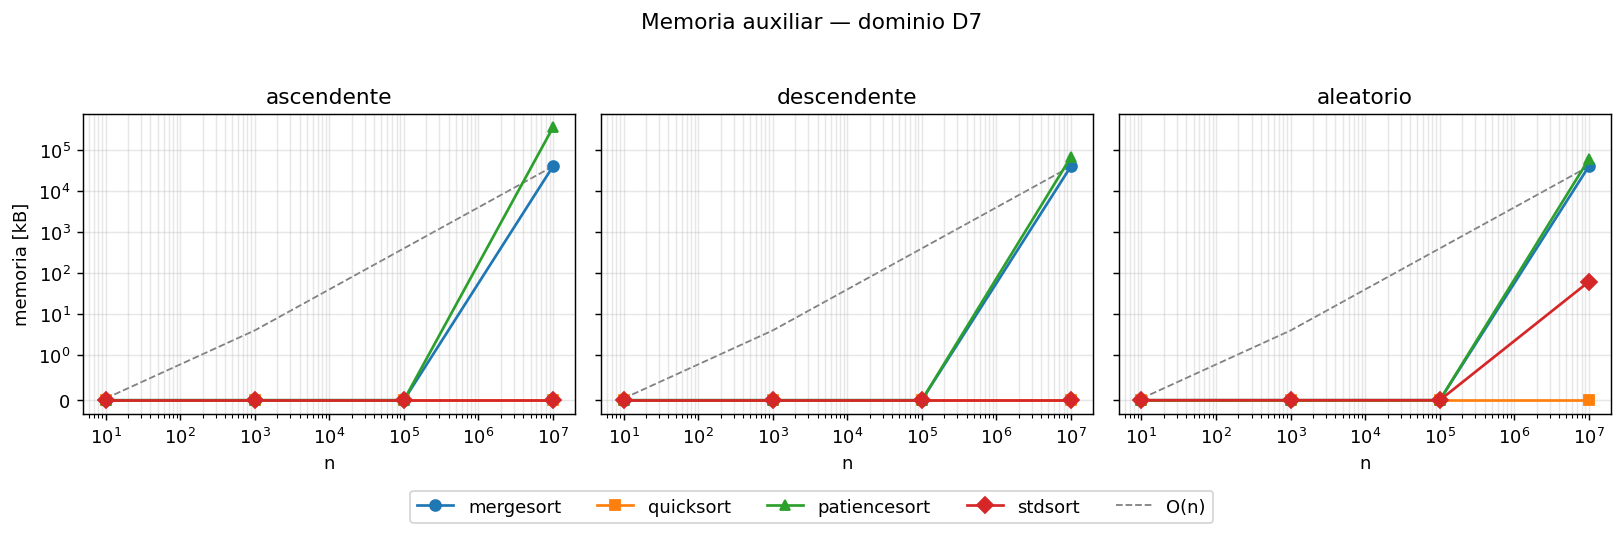
\includegraphics[width=0.95\textwidth]{sections/plots/sorting_memoria_D7.png}
    \caption{Memoria auxiliar (pico de RSS menos línea base) de los algoritmos
    de ordenamiento en $D_7$. Escala \emph{symlog}: los algoritmos in-place se
    dibujan sobre el eje.}
    \label{fig:sort_mem_d7}
\end{figure}

\begin{table}[H]
    \centering
    \begin{tabular}{l|rl}
        Algoritmo & Memoria aux. [kB] & Complejidad esperada \\ \hline
        QuickSort & 0 & $O(\log n)$ (pila) \\
        \texttt{std::sort} & 60 & $O(\log n)$ \\
        MergeSort & 38\,912 & $O(n)$ \quad ($\approx n\cdot 4$ B) \\
        PatienceSort & 58\,240 & $O(n)$ \quad ($\approx 1.5\,n$) \\
    \end{tabular}
    \caption{Memoria auxiliar a $n=10^7$, entrada aleatoria, dominio $D_7$.}
    \label{tab:sort_mem}
\end{table}

La \cref{fig:sort_mem_d7} y la \cref{tab:sort_mem} muestran dos grupos claros. QuickSort y \texttt{std::sort} operan in-place y su memoria auxiliar es prácticamente nula. Merge Sort y Patience Sort crecen linealmente con $n$: Merge necesita el arreglo auxiliar de la mezcla ($\approx n\cdot 4$ bytes) y Patience almacena las pilas ($\approx 1.5\,n$). Los valores medidos coinciden con la complejidad espacial teórica de cada algoritmo.

\subsection{Multiplicación de matrices}

Tanto el algoritmo naïve como Strassen \cite{strassen1969} se tomaron de GeeksforGeeks \cite{gfg_strassen}.

\begin{figure}[H]
    \centering
    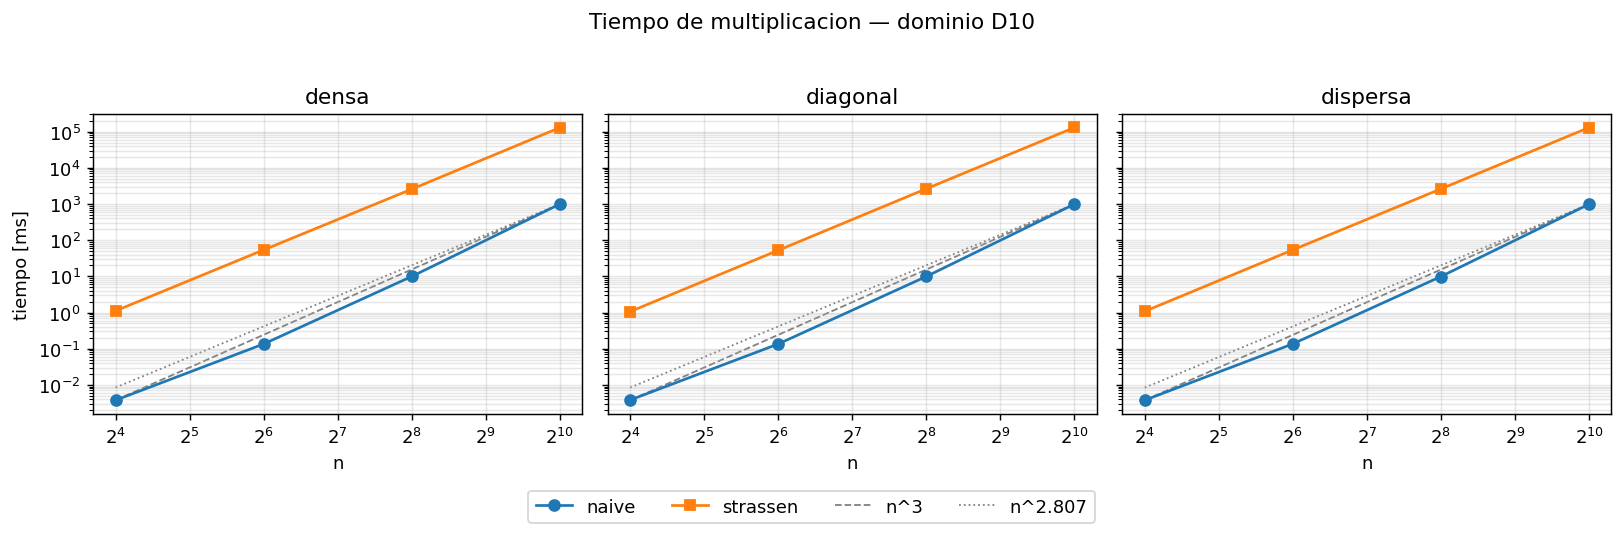
\includegraphics[width=0.95\textwidth]{sections/plots/matriz_tiempo_D10.png}
    \caption{Tiempo de multiplicación de matrices en el dominio
    $D_{10} = \{0,\dots,9\}$, por tipo de matriz. Escala log--log; referencias
    $n^3$ y $n^{2.807}$.}
    \label{fig:mat_time}
\end{figure}

\begin{table}[H]
    \centering
    \begin{tabular}{r|rr|rr|r}
        $n$ & Naïve [ms] & Strassen [ms] & Naïve mem [kB] & Strassen mem [kB] & Ratio \\ \hline
        $2^4$ & 0.004 & 1.12 & 0 & 0 & $296\times$ \\
        $2^6$ & 0.14 & 53.97 & 0 & 0 & $399\times$ \\
        $2^8$ & 9.97 & 2\,581 & 0 & 0 & $259\times$ \\
        $2^{10}$ & 995 & 129\,718 & 3\,849 & 49\,841 & $130\times$ \\
    \end{tabular}
    \caption{Multiplicación de matrices, tipo densa, dominio $D_{10}$. El tipo
    (densa / diagonal / dispersa) no altera los resultados.}
    \label{tab:mat}
\end{table}

En \cref{fig:mat_time} y \cref{tab:mat} el algoritmo naïve sigue la referencia $n^3$, mientras que Strassen queda unos dos órdenes de magnitud por encima pero con pendiente algo menor. A $n=1024$, naïve tarda 1 s y Strassen 130 s. El factor de crecimiento al duplicar $n$ es $7.0 / 6.9 / 7.1$ para Strassen (muy cercano al $7$ que corresponde a $n^{\log_2 7} = n^{2.807}$) y $6.0 / 8.6 / 10.0$ para naïve (en torno al $8$ de $n^3$). Es decir, Strassen \emph{sí} tiene la mejor complejidad asintótica y se observa en la pendiente, pero su constante lo hace $130$ veces más lento: el \emph{ratio} baja de $296\times$ a $130\times$ al crecer $n$, la curva converge, pero el punto de cruce está fuera de todo rango práctico. La constante proviene de copiar los \texttt{std::vector} anidados que representan las matrices y de pasar las submatrices por valor en cada uno de los siete productos recursivos.

Dos observaciones adicionales. Primero, naïve crece \emph{más} rápido que $n^3$ entre $2^8$ y $2^{10}$ ($\times 10$ por duplicación): a $n=1024$ cada matriz ocupa 4 MB y las tres no caben cómodamente en la caché L3 (16 MB), lo que aumenta los fallos de caché (un efecto que la notación asintótica no captura). Segundo, el tipo de matriz (densa, diagonal o dispersa) no cambia los tiempos: ambos algoritmos operan sobre almacenamiento denso y no aprovechan la estructura.
